\documentclass{beamer}
\usepackage[utf8]{inputenc}
\usepackage{caption}
\usepackage{etoolbox}
\usepackage{graphicx}
\usepackage{hyperref}
\usepackage{listings}
\usepackage{tikz}
\usetikzlibrary{arrows,positioning}

\newtoggle{GOODIES}
\toggletrue{GOODIES}
%\togglefalse{GOODIES}

\usetheme{Singapore}
% hide navigation symbols
\setbeamertemplate{navigation symbols}{}

\AtBeginSection[]
{
  \begin{frame}
    \frametitle{Source Code Management}
    \tableofcontents[currentsection]
  \end{frame}
}

\captionsetup[lstlisting]{font={small,tt}}

\lstset{
  basicstyle=\tiny\ttfamily,
  frame=single,
  captionpos=t,
}


\title{Git brunch!}
\subtitle{SCM for the modern developer}
\author{\href{mailto://virtualtam@flibidi.net}{Aurélien Tamisier}}
\institute{The Internet}

\begin{document}
\frame{\titlepage}

\section{Collaborative software}
\stepcounter{subsection}
\begin{frame}
  \frametitle{Archiving your work (1)}

  What's a software made of?
  \begin{itemize}
    \item specifications
    \item architecture \& design
    \item sources
    \item deliverables
  \end{itemize}
\end{frame}

\begin{frame}
  \frametitle{Archiving your work (2)}

  What do sources consist of?
  \begin{itemize}
    \item code
      % the very core of the software
    \item code comments
      % additional / internal info: how do things work?
    \item build metadata
      % external dependencies
      % build instructions
      % packaging info
    \item developer documentation
      % README, licensing
  \end{itemize}
  \begin{block}{Notice anything?}
    These all are text files! % Hurray!
  \end{block}
\end{frame}

\begin{frame}
  \frametitle{Garageware: single developer}

  ``AaD, I am...''
  \begin{itemize}
    \item working on a small-sized project...
      % whether it's a script, hack, utility
    \item making backups of my work from time to time...
      % because you're obviously making backups, right?
    \item ... keeping copies here and there...
      % like, in your grandma's mailbox, or, like, in your goldfish's Dropbox
      % repository... whatever
    \item ... and quite happy with it, thanks! ;-)
  \end{itemize}
  \begin{alertblock}{Alert! Computer crash!}
    Er... \textit{v1.3.125\_test3.zip}, this is the good one, right?
  \end{alertblock}
\end{frame}

\begin{frame}
  \frametitle{Once upon a time, in a small team}

  2+ nice lads working on the same piece of software... of course:
  \begin{itemize}
    \item we'll \textit{al-way-s} be working on different code sections
    \item or even better, different source files!
    \item there'll never be any conflict...
    \item and everyone will be happily compiling ever after...
  \end{itemize}
  \begin{block}{Software is no fairy tale}
    Sorry to disappoint, really...
  \end{block}
\end{frame}

\iftoggle{GOODIES}{
  \begin{frame}
    \frametitle{\$ svn commit -{}-force}
    \begin{center}
      
\includegraphics[width=0.8\textwidth]{img/notdistributed.jpg}
    \end{center}
  \end{frame}
}{}

\begin{frame}
  \frametitle{What about a company?}

  Dozens of developers, from several teams:
  \begin{itemize}
    \item working on shared projects
      % 'cause you don't duplicate libs, do you?
    \item modifying the same sources...
    \item ... to serve different purposes
      % features, OS, clients...
  \end{itemize}
  \begin{block}{(Not-so) straightforward solutions}
    \begin{itemize}
      \item versioning hell: duplicate everything
      \item integration hell: designate a \textless \textit{project\_name} \textgreater guru
    \end{itemize}
  \end{block}
\end{frame}

\begin{frame}
  \frametitle{Same code, different delivery flavours}

  Given
  \begin{itemize}
    \item three features \textit{f1, f2, f3}
    \item three clients \textit{A, B, C}
  \end{itemize}
  You may want to provide:
  \begin{itemize}
    \item A: f1, f2, f3
    \item B: f1, f3
    \item C: f2, and a customized f3
  \end{itemize}
  \begin{exampleblock}{Real-world example}
    Web Content Management Systems (CMS): Wordpress, Drupal, MediaWiki...
  \end{exampleblock}
\end{frame}

\begin{frame}
  \frametitle{Getting social}

  We need flexible tools to:
  \begin{itemize}
    \item manage source code
    \item keep track of released versions
    \item allow collaborative work
    \item deliver customized products
  \end{itemize}
  \begin{block}{There comes...}
    \textbf{S}ource \textbf{C}ode \textbf{M}anagement,
    a.k.a. \textbf{V}ersion \textbf{C}ontrol \textbf{S}ystem
  \end{block}
\end{frame}

\section{Git}
\stepcounter{subsection}
\begin{frame}{About Git}
  \begin{itemize}
    \item Linus Torvalds, 2005
    \item Linux kernel sources
    \item distributed
    \item focus on data integrity \& performance
    \item popularized by GitHub
  \end{itemize}
  \begin{block}{Other distributed SCMs}
    Mercurial (hg), GNU Bazaar (bzr), Fossil
  \end{block}
\end{frame}

\begin{frame}{Git repositories (1)}
  Git is a distributed SCM, which means:
  \begin{itemize}
    \item every working copy \textit{(fork)} -either local or distant-
      is itself a fully functional repository
    \item any repository holds a complete history (for a given branch)
    \item developments may happen across various networks/communities
    \item easy to keep track of upstream changes
  \end{itemize}
\end{frame}

\begin{frame}{Commits}
  \begin{itemize}
    \item code changes are stored as \textit{commits}
    \item a commit contains
      \begin{itemize}
        \item a description: what has been modified?
        \item context information: author, signature, etc.
        \item the actual code changes (diff)
      \end{itemize}
    \item and is identified by a unique \textit{revision} (SHA-1)
    \item commits are \textit{local} objects, and contain changes locally
      \textit{staged} until they are \textit{pushed} to a remote repository
      (if any)
      % ain't it subversive?
  \end{itemize}
\end{frame}

\begin{frame}{Branches}
  Branching is the essence of distributed SCMs
  \begin{itemize}
    \item any branch is a working copy
    \item creation, merging and deletion are cheap operations
    \item analogy: pointers, chained lists
      \begin{itemize}
        \item a commit points to its parent commit
        \item a branch is a pointer to a given revision (commit)
        \item a repository's \textit{head} refers to the most recent
          commit of an existing branch
      \end{itemize}
  \end{itemize}
\end{frame}

\begin{frame}{Branching example 1}
  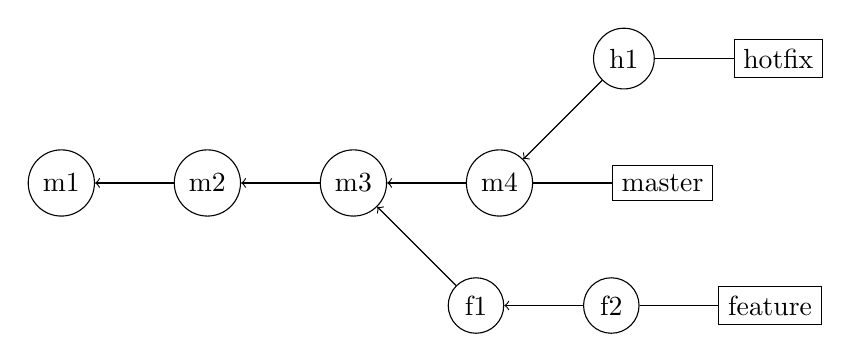
\begin{tikzpicture}
    % simple branching example
    \tikzset{commit/.style = {shape=circle,draw}}
    \tikzset{label/.style = {shape=rectangle,draw}}
    \tikzset{pre/.style = {->}}

    % master
    \node[commit] (m1)                 {m1};
    \node[commit] (m2) [right=of m1]   {m2}
       edge [pre] (m1);
    \node[commit] (m3) [right=of m2]   {m3}
       edge [pre] (m2);
    \node[commit] (m4) [right=of m3]   {m4}
       edge [pre] (m3);
    \node[label]  (master) [right=of m4] {master}
       edge (m4);

    % hotfix branch
    \node[commit] (h1) [above right=of m4]   {h1}
       edge [pre] (m4);
    \node[label]  (hotfix) [right=of h1] {hotfix}
       edge (h1);

    % feature branch
    \node[commit] (f1) [below right=of m3]   {f1}
       edge [pre] (m3);
    \node[commit] (f2) [right=of f1]   {f2}
       edge [pre] (f1);
    \node[label]  (feature) [right=of f2] {feature}
       edge (f2);
  \end{tikzpicture}
\end{frame}

\begin{frame}{Branching example 2}
  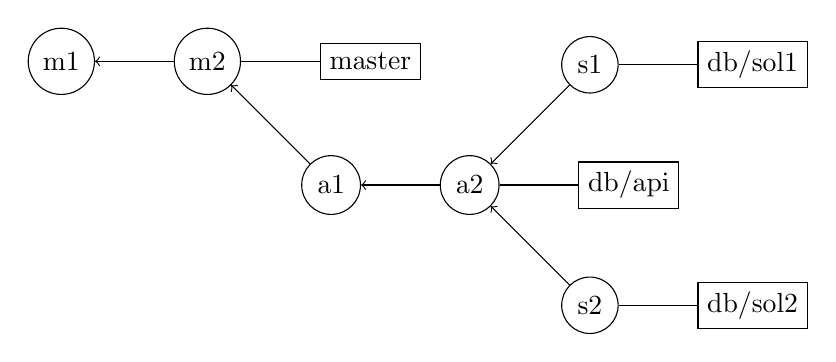
\begin{tikzpicture}
    % common use case: experimenting with stuff
    % - base api / interfaces
    % - 2 potential solutions
    \tikzset{commit/.style = {shape=circle,draw}}
    \tikzset{label/.style = {shape=rectangle,draw}}
    \tikzset{pre/.style = {->}}

    % master
    \node[commit] (m1)                 {m1};
    \node[commit] (m2) [right=of m1]   {m2}
       edge [pre] (m1);
    \node[label]  (master) [right=of m2] {master}
       edge (m2);

    % api / interfaces
    \node[commit] (a1) [below right=of m2]   {a1}
        edge [pre] (m2);
    \node[commit] (a2) [right=of a1]   {a2}
        edge [pre] (a1);
    \node[label]  (api) [right=of a2] {db/api}
        edge (a2);

    % solution 1
    \node[commit] (s1) [above right=of a2]   {s1}
        edge [pre] (a2);
    \node[label]  (sol1) [right=of s1] {db/sol1}
        edge (s1);

    % solution 2
    \node[commit] (s2) [below right=of a2]   {s2}
        edge [pre] (a2);
    \node[label]  (sol2) [right=of s2] {db/sol2}
        edge (s2);

  \end{tikzpicture}
\end{frame}

\iftoggle{GOODIES}{
  \begin{frame}{Branches are cool!}
    \begin{center}
      % OMG!!!
      
\includegraphics[width=0.6\textwidth]{img/omgabranch.jpg}
      % A BRANCH!!!
    \end{center}
  \end{frame}
}{}

\begin{frame}{Git repositories (2): remotes}
  \begin{itemize}
    \item \textit{remote}: alias for a parent repository,
      either local or distant
    \item any number of remotes can be added
  \end{itemize}
  \begin{block}{Use cases}
    GitHub workflow, development outsourcing
  \end{block}
\end{frame}

\begin{frame}{Git commands (1): commit changes}
  \begin{description}
    \item[git add] \hfill \\
      stage changes to include them in the next commit
    \item[git clean] \hfill \\
      remove undesired (unversioned, ignored) changes
    \item[git rm] \hfill \\
      delete and unversion files
    \item[git commit] \hfill \\
      create a commit from staged changes
    \item[git commit -s] \hfill \\
      create a signed commit
    \item[git commit -{}-amend] \hfill \\
      alter the last commit: add/remove/modify files
  \end{description}
\end{frame}

\begin{frame}{Git commands (2): branches}
  \begin{description}
    \item[git branch] \hfill \\
      create \& delete branches
    \item[git tag] \hfill \\
      create \& delete tags
    \item[git pull] \hfill \\
      update branch information
    \item[git push remote branch] \hfill \\
      push local commits to a remote branch
    \item[git rebase remote/branch] \hfill \\
      rebase the current branch
    \item[git reset -{}-hard revision] \hfill \\
      reset the current branch to a reference revision
  \end{description}
\end{frame}

\begin{frame}{Git commands (3): checkout, the all-in-one}
  \begin{description}
    \item[git checkout revision] \hfill \\
      checkout a given revision: branch, tag, commit ID...
    \item[git checkout revision file1 file2...] \hfill \\
      checkout the selected files on a given revision
    \item[git checkout -{}- file1 file2...] \hfill \\
      unstage changes for the selected files
    \item[git checkout revision -b branch] \hfill \\
      create a branch from a given revision, and checkout it
  \end{description}
\end{frame}

\begin{frame}{Git commands (4): information}
  \begin{description}
    \item[git diff] \hfill \\
      show unstaged changes
    \item[git diff revision] \hfill \\
      show the differences with a given revision
    \item[git log] \hfill \\
      display the commit history
    \item[git show revision] \hfill \\
      show the commit message and the diff
    \item[git status] \hfill \\
      display local commits, unversioned changes...
  \end{description}
\end{frame}

\begin{frame}[fragile]{Example: basic Git configuration}
  \begin{columns}[t]
    \begin{column}{0.5\textwidth}
      \lstinputlisting[caption=\~{}/.gitconfig]{examples/simple/gitconfig}
    \end{column}
    \begin{column}{0.5\textwidth}
      \lstinputlisting[caption=\~{}/.ssh/config]{examples/simple/ssh_config}
    \end{column}
  \end{columns}
\end{frame}

\section{Repo \& Gerrit}
\stepcounter{subsection}
\begin{frame}{About Repo}
  \begin{itemize}
    \item Google, 2008
    \item Android Open Source Project (AOSP)
    \item tool for managing multiple Git repositories
    \item integrates with Gerrit (Code Review)
  \end{itemize}
\end{frame}

\begin{frame}{Running batch tasks}
  Usual Repo workflow:
  \begin{itemize}
    \item create a feature branch over several repositories
    \item edit code across repositories to make the feature work
    \item commit the changes
    \item upload changes to Gerrit:
      \begin{itemize}
        \item creates one patch per commit
        \item several \textit{local} commits on the same repository are uploaded
          as a series of dependent patches (on the same topic-branch)
      \end{itemize}
    \item code review happens ;-)
  \end{itemize}
\end{frame}

\begin{frame}{Repo commands (1)}
  \begin{description}
    \item[repo init -u url -m manifest] \hfill \\
      initialize a Repo workspace using a repository containing XML manifests
    \item[repo sync] \hfill \\
      update all repositories with upstream changes
    \item[repo start topic\_branch repo1] \hfill \\
      start a topic-branch on a given repository
    \item[repo upload] \hfill \\
      submit local commits to Gerrit
    \item[repo rebase] \hfill \\
      rebase a topic-branch on the mainline
  \end{description}
\end{frame}

\begin{frame}{Repo commands (2)}
  \begin{description}
    \item[repo status] \hfill \\
      status for local repositories
    \item[repo prune topic\_branch] \hfill \\
      destroy a topic-branch
    \item[repo forall -c "command"] \hfill \\
      iterate on repositories, execute a (series of) command
    \item[repo forall -c "git clean -xdf; git reset -{}-hard HEAD"] \hfill \\
      efficient workspace cleanup before running \texttt{repo sync}
  \end{description}
\end{frame}

\begin{frame}{git-review}
  A lightweight alternative to Repo:
  \begin{itemize}
    \item installs a Git hook to add a Change-Id
    \item adds the \textit{git review} subcommand
    \item eases submitting to and cherry-picking from Gerrit
  \end{itemize}  
  \begin{description}
    \item[git review] \hfill \\
      submit local commits to Gerrit
    \item[git review -l] \hfill \\
      list incoming reviews on the current repository
    \item[git review -d patch] \hfill \\
      cherry-picks a Gerrit patch in a new branch
  \end{description}
\end{frame}

\begin{frame}[fragile]{Example: Git/Gerrit configuration}
  \begin{columns}[t]
    \begin{column}{0.5\textwidth}
      \lstinputlisting[caption=\~{}/.gitconfig]{examples/review/gitconfig}
    \end{column}
    \begin{column}{0.5\textwidth}
      \lstinputlisting[caption=\~{}/.ssh/config]{examples/review/ssh_config}
    \end{column}
  \end{columns}
\end{frame}


\begin{frame}{Questions}
  \begin{columns}[t]
    \begin{column}{0.4\textwidth}
      Thanks for your attention!

      Now's time for:
      \begin{itemize}
      \item Q \& A
      \item Demo!
      \end{itemize}
    \end{column}
    \iftoggle{GOODIES}{
      \begin{column}{0.6\textwidth}
        \begin{center}
          
\includegraphics[width=\textwidth]{img/gitgrumpy.jpg}
        \end{center}
      \end{column}
    }{}
  \end{columns}
\end{frame}

%\appendix
%\section{Resources}
\stepcounter{subsection}
\begin{frame}
  \frametitle{Git resources}
  \begin{itemize}
    \item \url{http://git-scm.com}
    \item \url{http://www.cheat-sheets.org/saved-copy/git-cheat-sheet.pdf}
    \item \url{http://docs.openstack.org/infra/manual/developers.html}
  \end{itemize}
\end{frame}

\begin{frame}
  \frametitle{Repo resources}
  \begin{itemize}
    \item \url{https://source.android.com/source/developing.html}
    \item \url{http://source.android.com/source/using-repo.html}
  \end{itemize}
\end{frame}

\begin{frame}
  \frametitle{Tools}
  \begin{itemize}
    \item \textit{.gitconfig} - customize your Git aliases!
    \item gitk - browse a Git repository (GUI)
    \item meld - view side-by-side diffs when merging and resolve conflicts (GUI)
  \end{itemize}
\end{frame}

\begin{frame}
  \frametitle{Advanced usage}
  \begin{itemize}
    \item \url{http://nvie.com/posts/a-successful-git-branching-model/}
    \item \url{http://durdn.com/blog/2012/11/22/must-have-git-aliases-advanced-examples/}
    \item \url{http://justinhileman.info/article/git-pretty/git-pretty.png}
    \item \url{http://git-scm.com/book/en/v2/Git-Basics-Undoing-Things}
    \item \url{https://code.google.com/p/gource/}
  \end{itemize}
\end{frame}

\end{document}
